\documentclass{article}
\usepackage[margin=1in]{geometry}
\usepackage{amsmath,amsthm,amssymb}
\usepackage{bbm,enumerate,mathtools}
\usepackage{tikz,pgfplots}
\usepackage{chessboard}
\usepackage[hidelinks]{hyperref}
\usepackage{multicol} % Problem 35

\newenvironment{question}{\begin{trivlist}\item[\textbf{Question.}]}{\end{trivlist}}
\newenvironment{note}{\begin{trivlist}\item[\textbf{Note.}]}{\end{trivlist}}
\newenvironment{references}{\begin{trivlist}\item[\textbf{References.}]}{\end{trivlist}}
\newenvironment{related}{\begin{trivlist}\item[\textbf{Related.}]\end{trivlist}\begin{enumerate}}{\end{enumerate}}


\begin{document}
\rating{3}{4}
Ron Graham's (A006255) sequence is the least k for which there exists a
strictly increasing sequence \[
  n = a_1 \leq a_2 \leq \hdots \leq a_T = k \text{ where }
  a_1 \cdot\hdots\cdot a_T \text{ is square.}
\]
A006255 is bounded above by A072905, the least $k > n$ such that $k\cdot n$
is square.
\begin{question}
  Does there exist any $n$ for which $A006255(n) = A072905(n)$. In other words,
  is there any nonsquare $n$ for which $n \cdot A006255(n)$ is square?
\end{question}

\begin{related}
  \item Does the gap $A072905(n) - A006255(n)$ have a nonzero lower bound?\\
    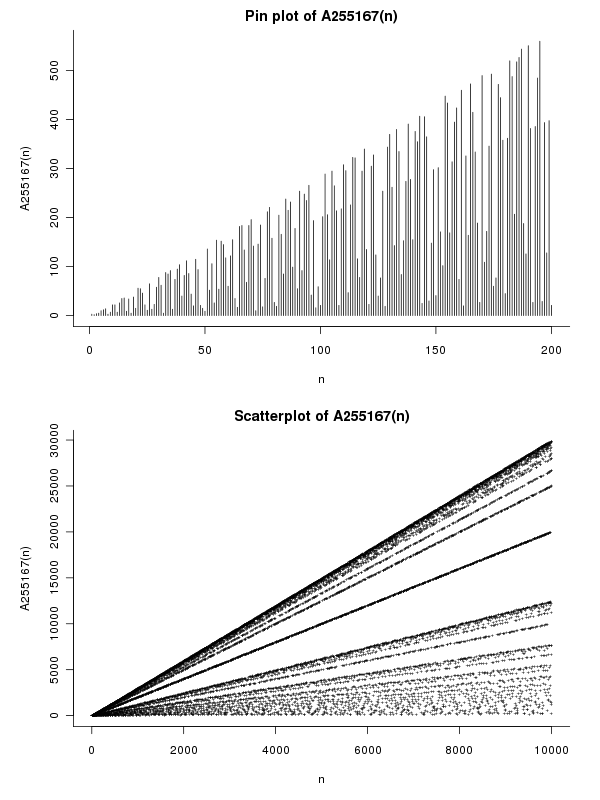
\includegraphics[trim={0cm 0 0 14cm},clip,scale=0.7]{assets/018_problem_A255167}
\end{related}

\begin{note}
  This is equivalent to showing that for any $a < b$ with the same
  squarefree part, there is some subset of $\{ a + 1, a + 2, \hdots, b - 1 \}$
  such that the product of the elements of the subset has the same squarefree
  part as $a$ (and $b$).
\end{note}

\begin{references}
  \item \url{https://oeis.org/A006255}
  \item \url{https://oeis.org/A072905}
  \item \url{https://oeis.org/A255167}
\end{references}
\end{document}
